\section{Uma Primeira Seção para o Apêndice}

A matriz de Dilema Linear $M$ e o vetor de torques inerciais $b$,
utilizados na simulação são calculados segundo a formulação 
abaixo:
\begin{equation}
M=\left[ \begin{array}{ccc}
M_{11} & M_{12} & M_{13} \\
M_{21} & M_{22} & M_{23} \\
M_{31} & M_{32} & M_{33}
\end{array} \right]
\end{equation}

\begin{figure}[h]
\centering
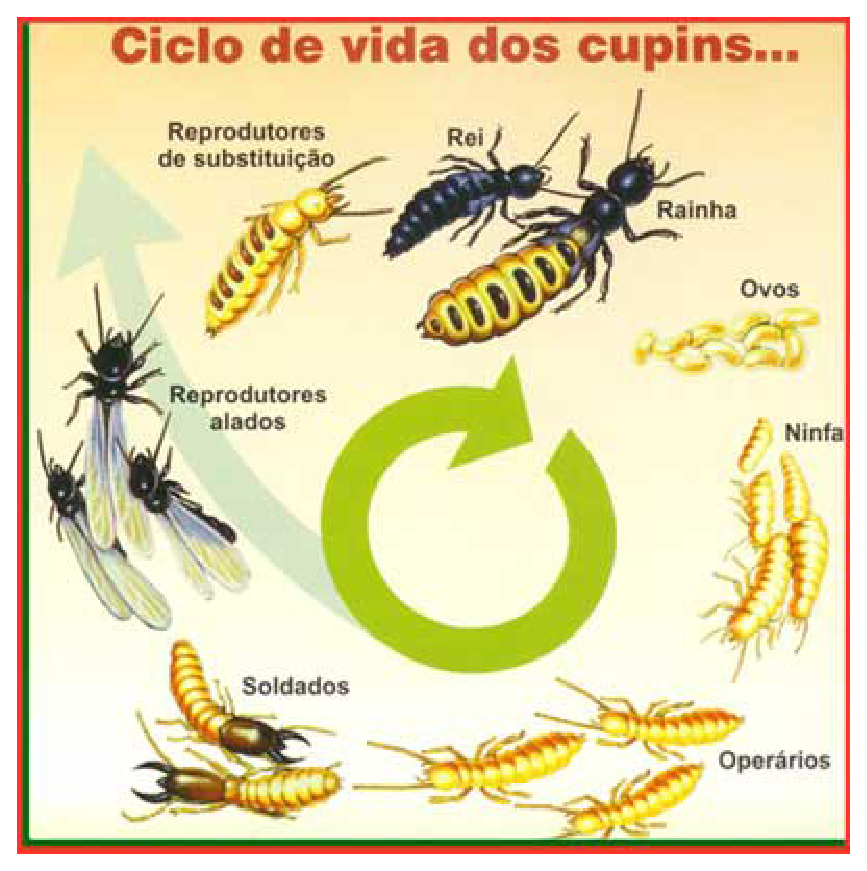
\includegraphics[height=5cm, width=5cm]{ApeA/pragas_ciclo_cupim}
\caption{Uma figura que está no apêndice}\label{FD}
\end{figure}
